%!TEX root = ../Pflichtenheft.tex

\chapter{Benutzeroberfläche}
\label{chap:ui}

\section{Haupseite und Buchung}

Die Haupseite der Anwendung ist in \ref{fig:hauptseite} dargestellt. Dabei haben UserInnen die Möglichkeit dem Raum zu buchen oder auf andere Ansichten zu wechseln.
Sollten NuterInnen eine Buchung vornehmen wollen, so klicken diese in den gewünschten Zeitraum und es wird der Dialog in \ref{fig:buchung} dargestellt. Hier können NutzerInnen die gewünschte Zeit und den Raum auswählen.
Tätigen NutzerInnen eine Buchung, so werden diese aufgefordert sich anzumelden. Dieser Dialog ist in \ref{fig:login} dargestellt. Alternativ ist dieses Dialog auch über den Login Button der in Abbildung \ref{fig:hauptseite} zu sehen ist, erreichbar.
Der Banner in allen Ansichten zeigt den aktuellen Raumstatus an. Insbesondere wird dabei die entsprechend Priorität durch die Farbe des Banners angezeigt.
Sind NutzerInnen eingeloggt und belegen den Raum so wird eine die in Abbildung \ref{fig:checkout} dargestellte Ansicht angezeigt. Hier können NutzerInnen den Raum wieder über den Quick-Checkout Button freigeben.

\begin{figure}[ht]
    \centering
    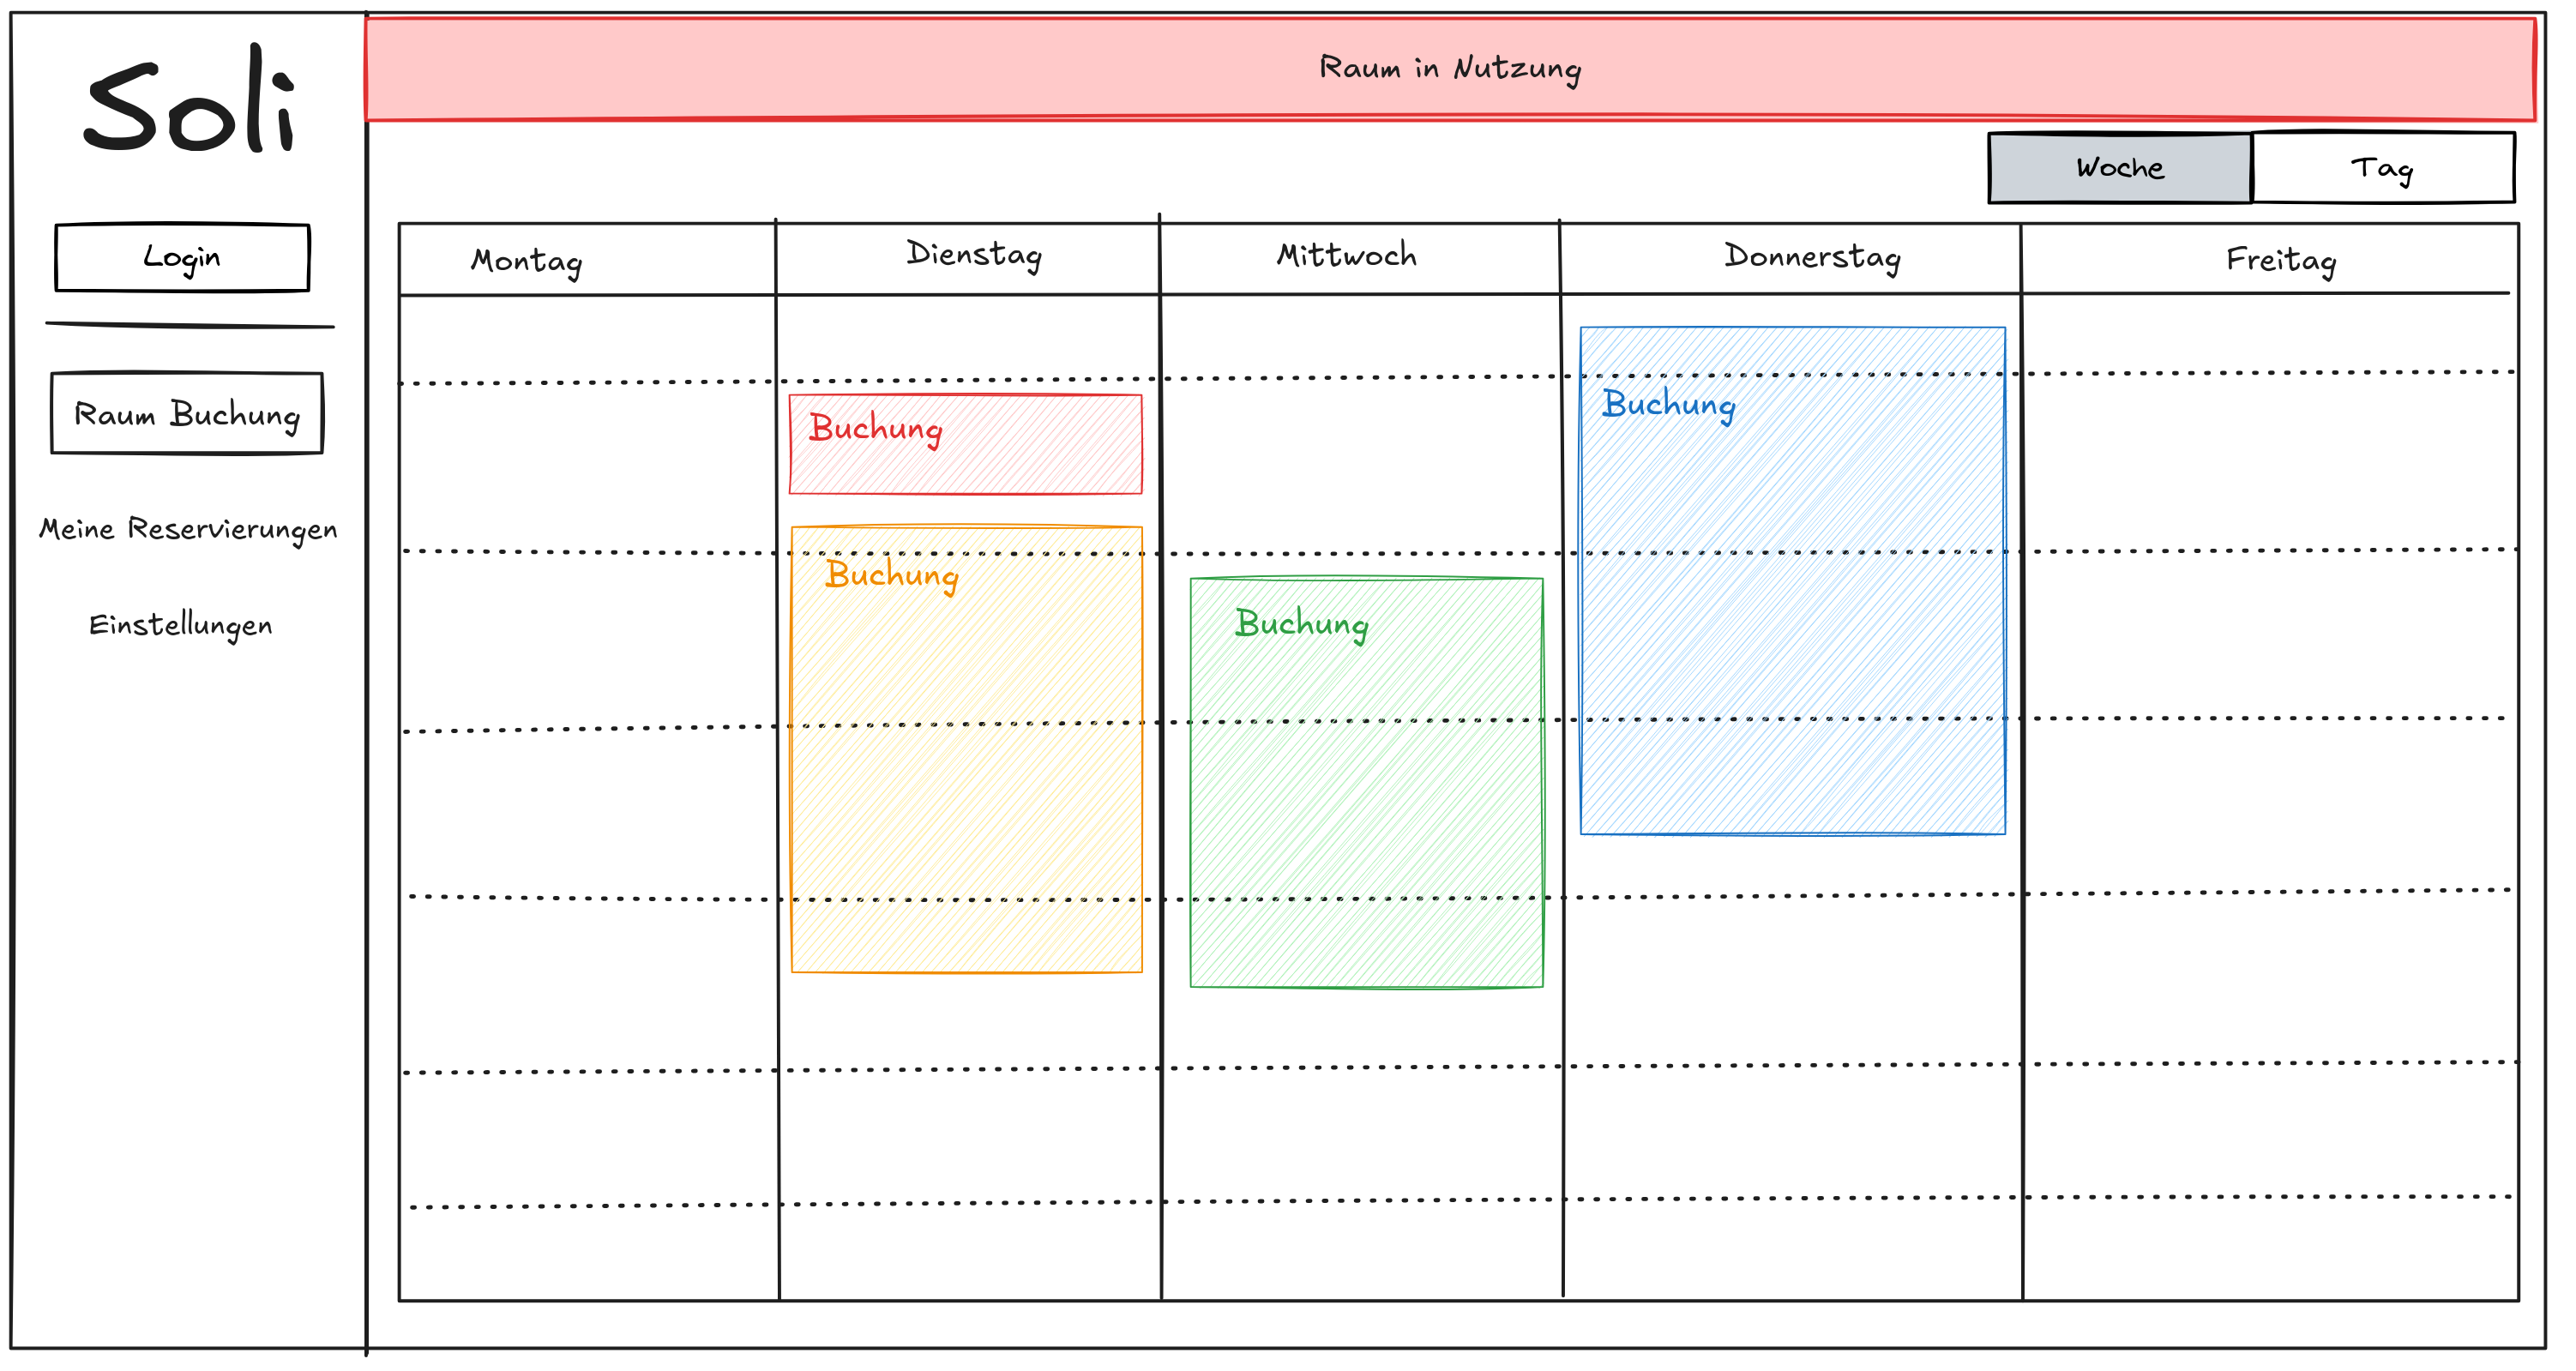
\includegraphics[scale=0.15]{figures/MainPageUI.png}
    \caption{Haupseite der Anwendung}
    \label{fig:hauptseite}
\end{figure}

\begin{figure}[ht]
    \centering
    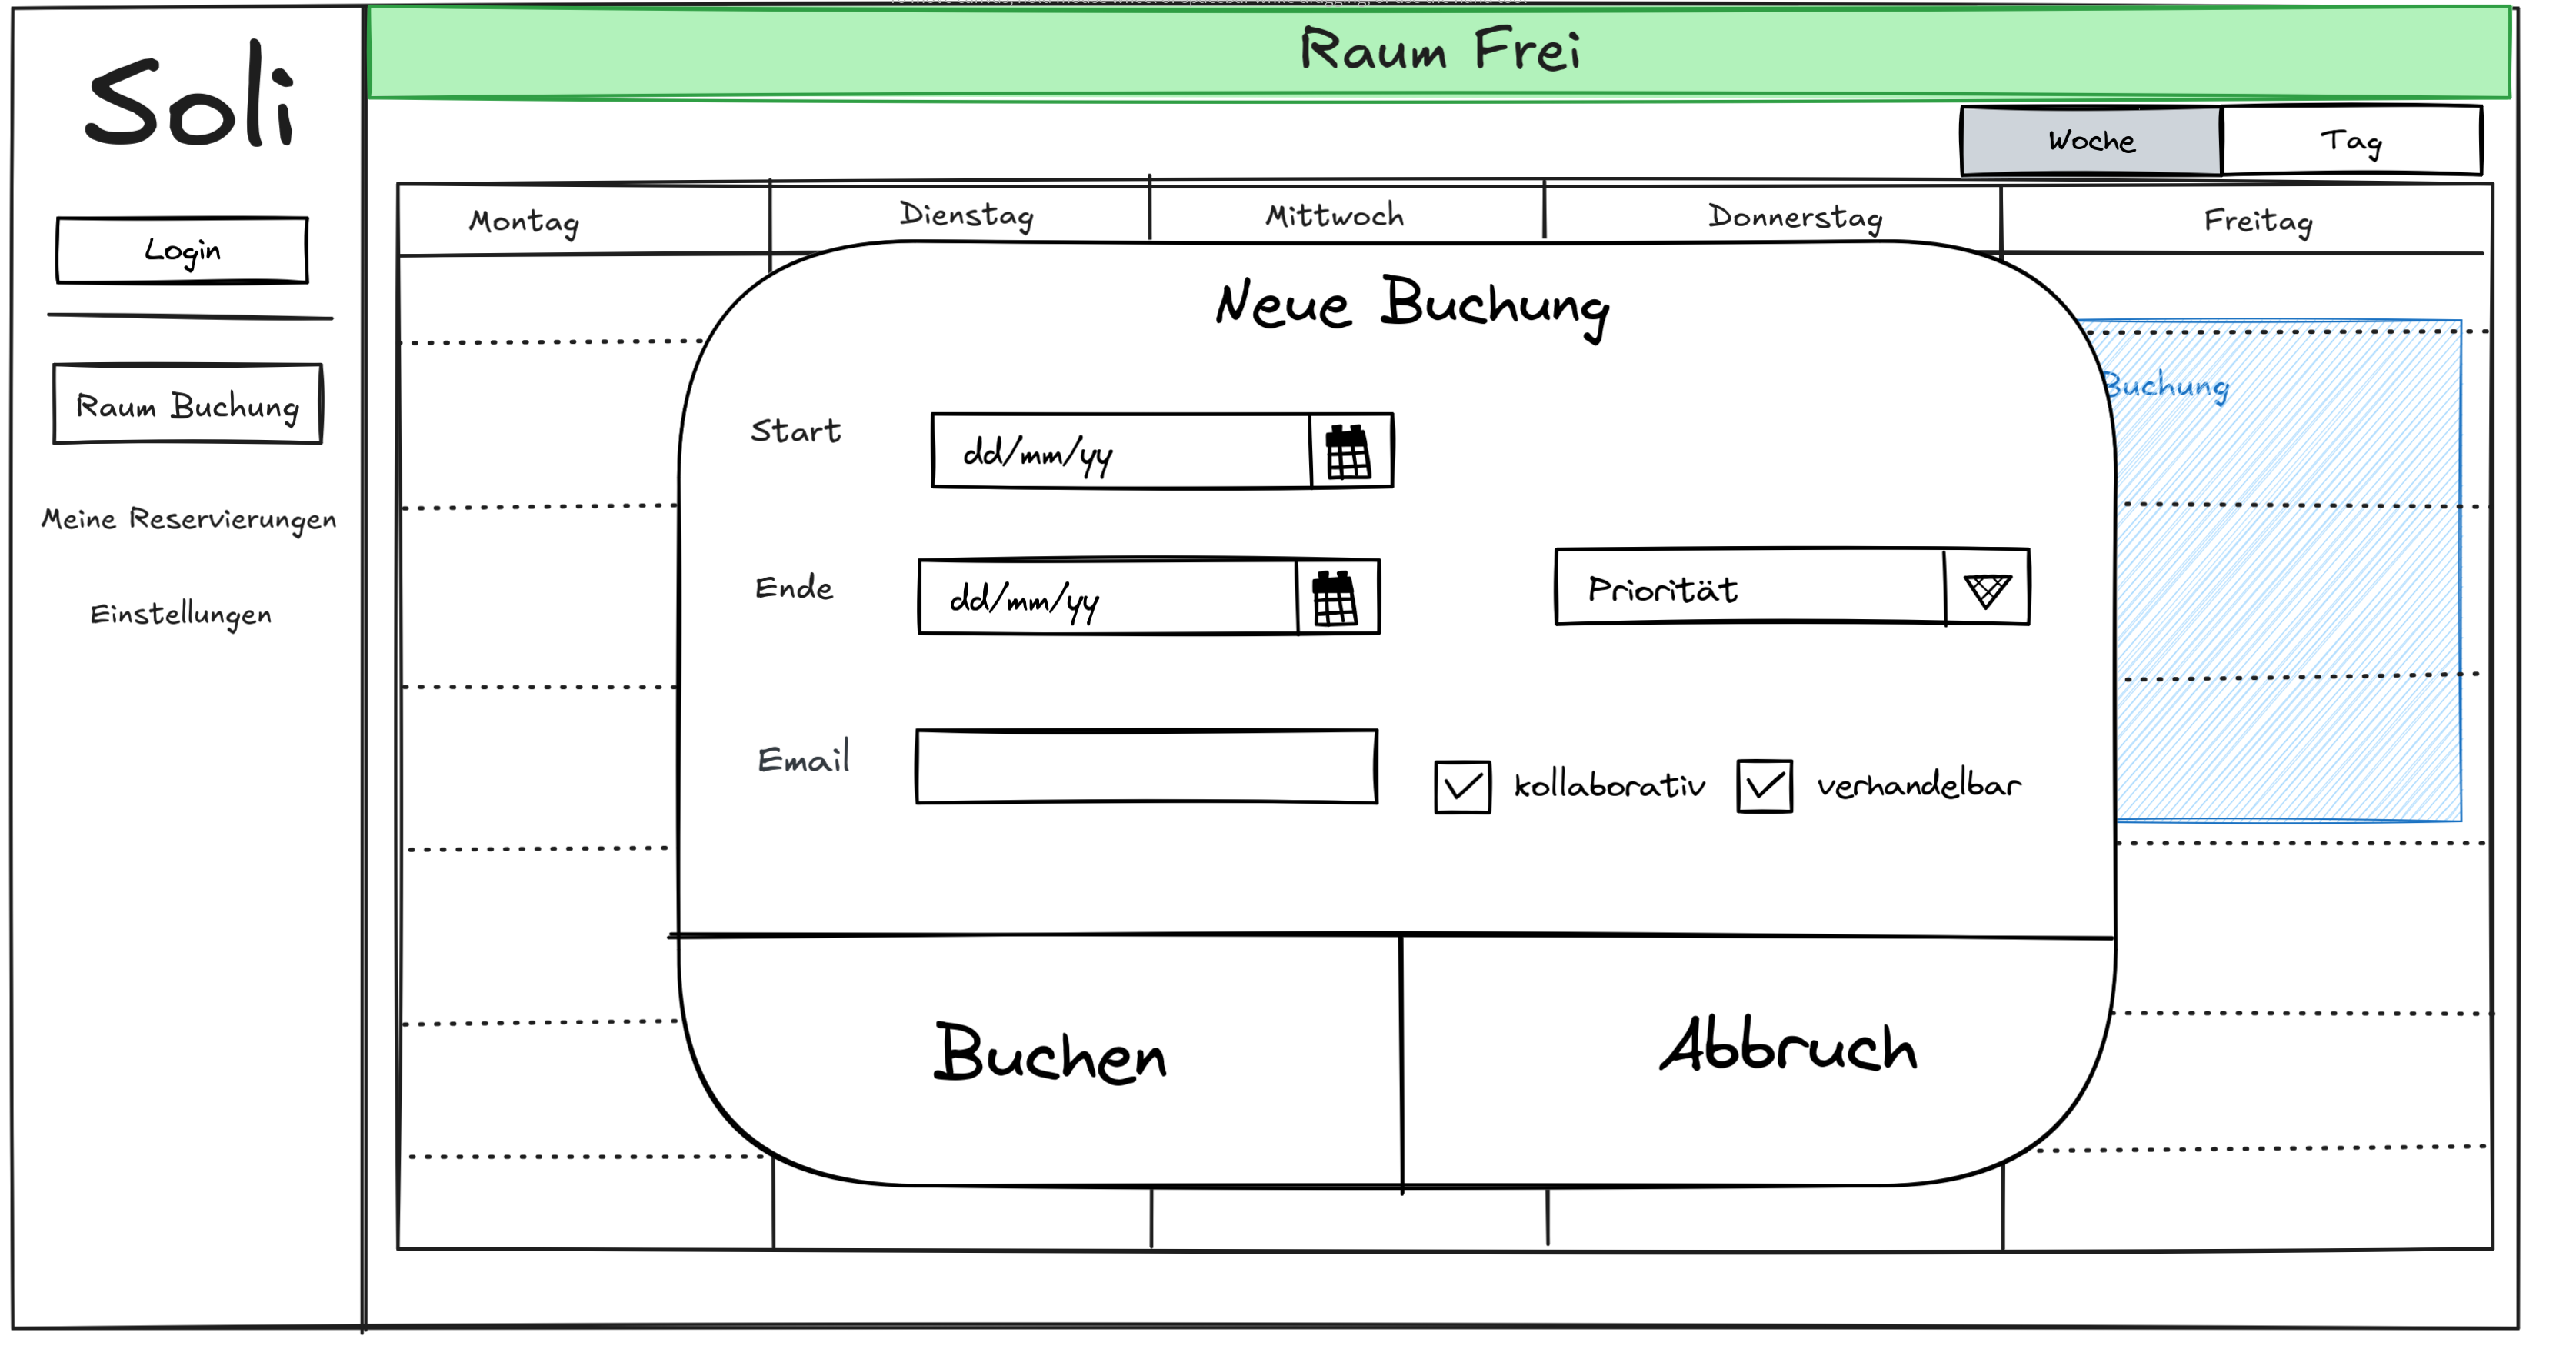
\includegraphics[scale=0.15]{figures/booking.png}
    \caption{Buchung des Raumes}
    \label{fig:buchung}
\end{figure}

\begin{figure}[ht]
    \centering
    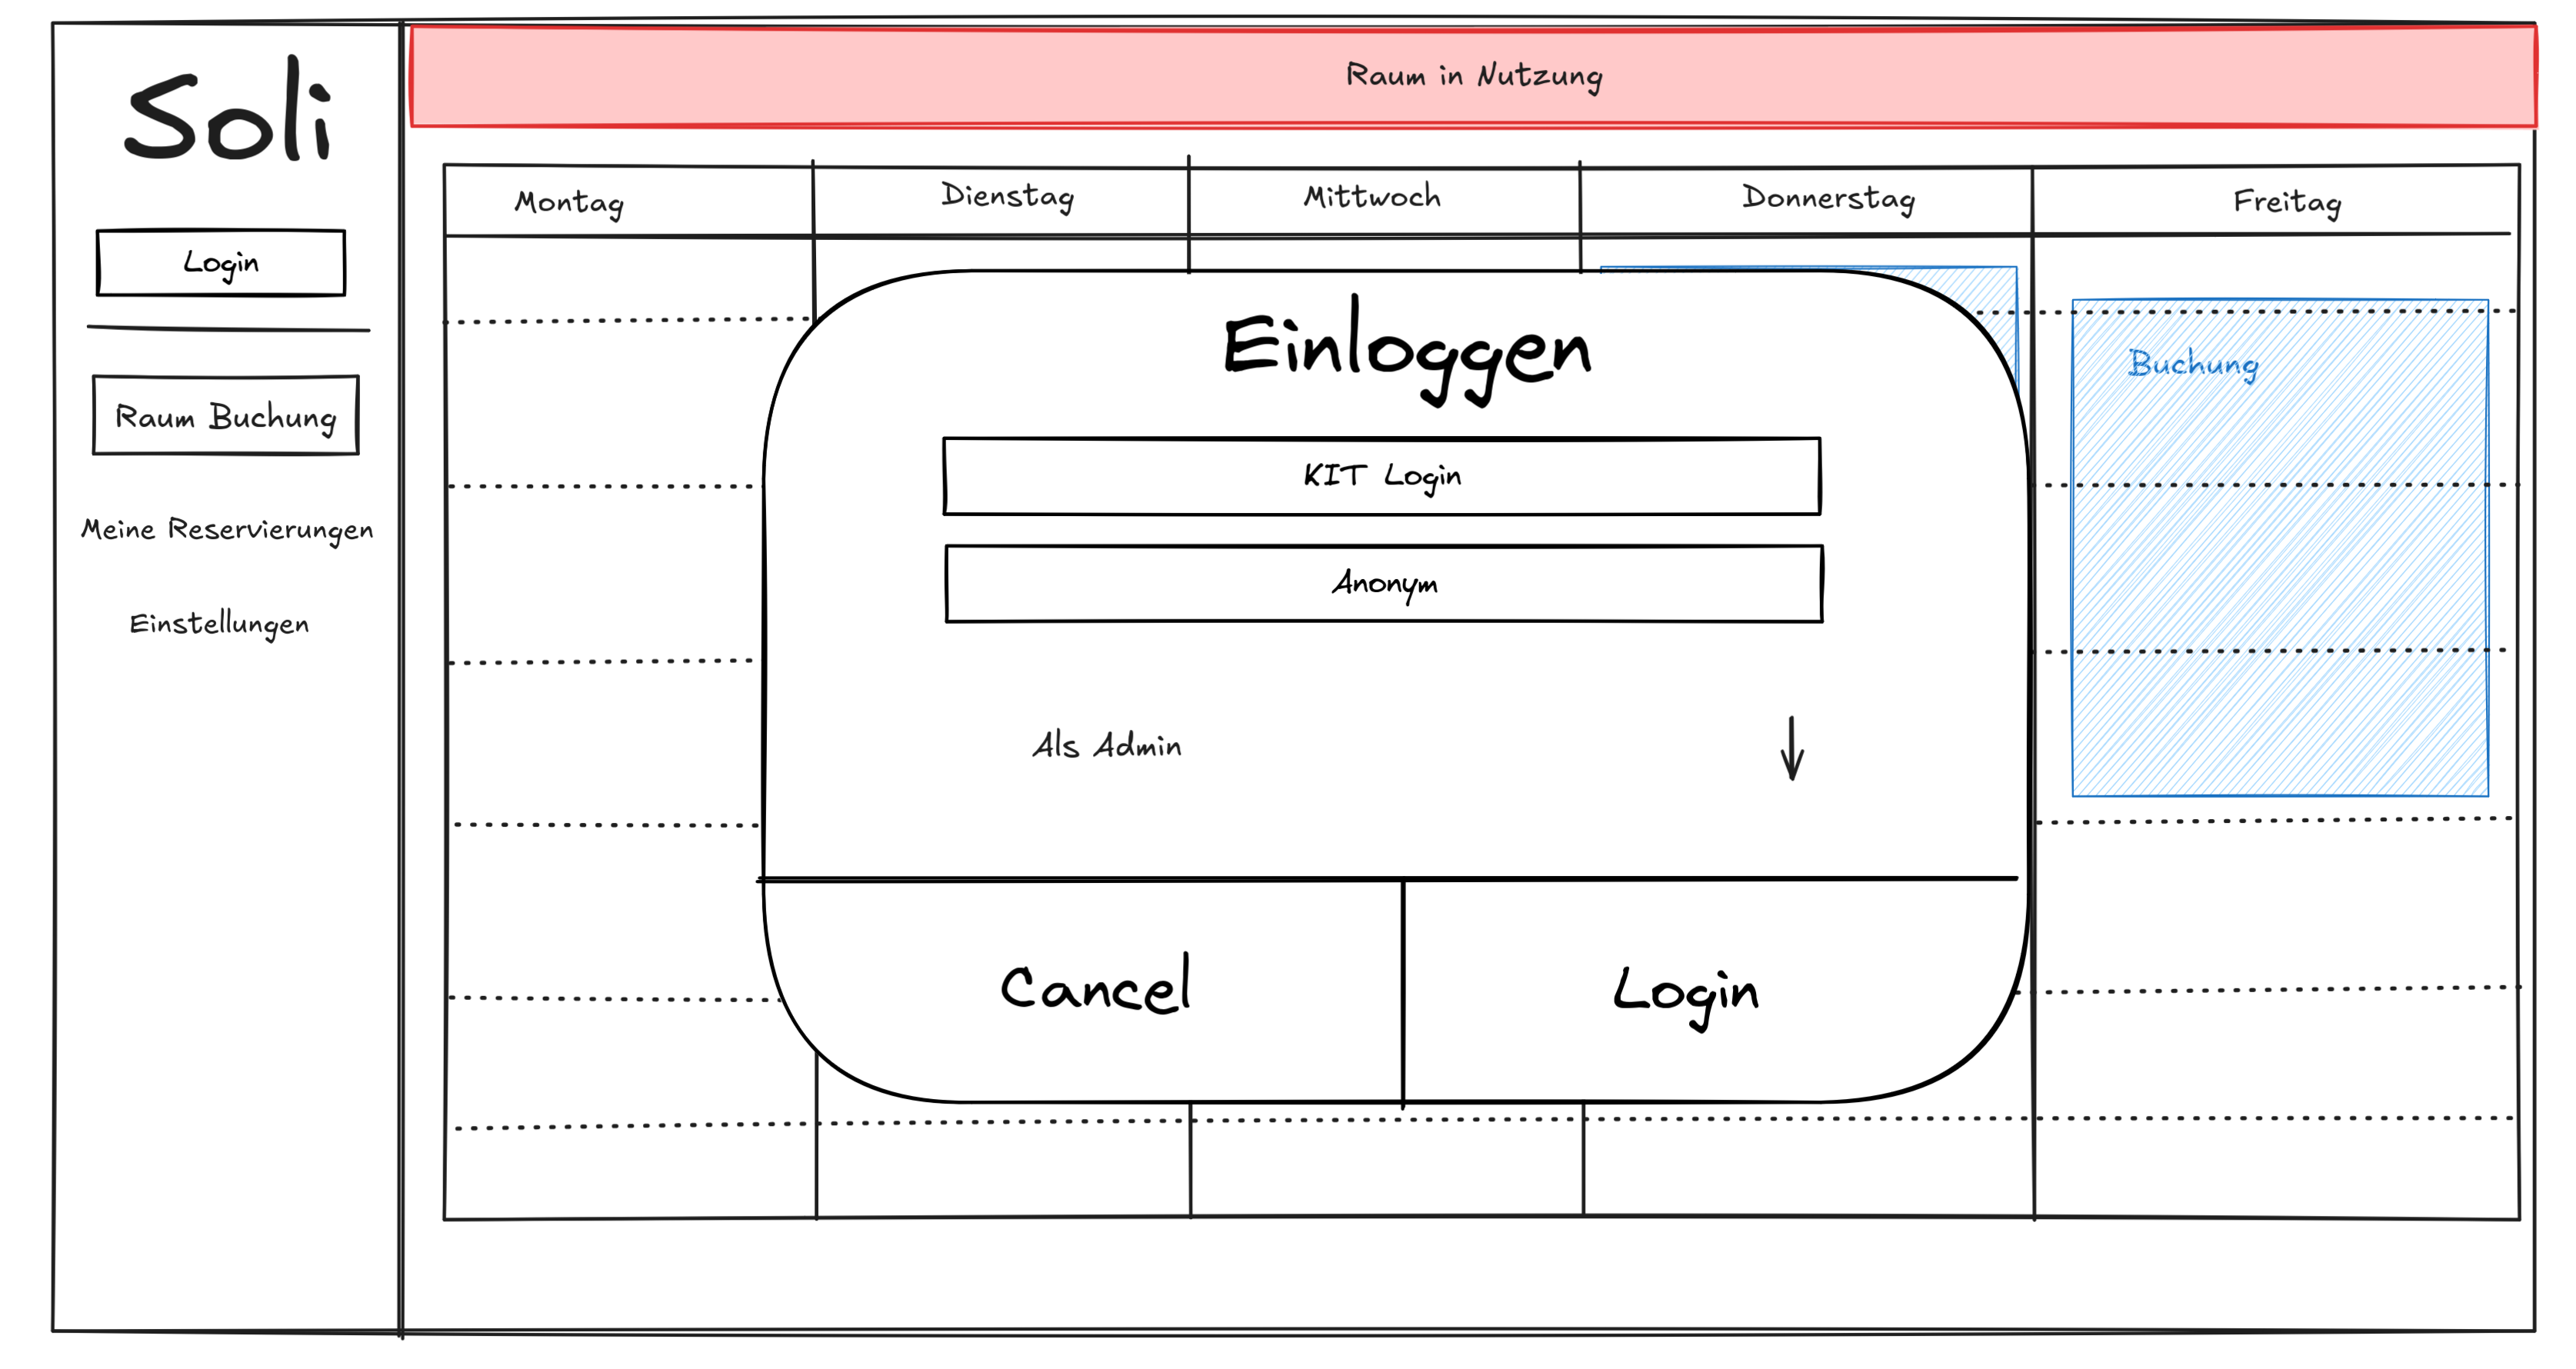
\includegraphics[scale=0.15]{figures/login.png}
    \caption{Login}
    \label{fig:login}
\end{figure}

\begin{figure}[ht]
    \centering
    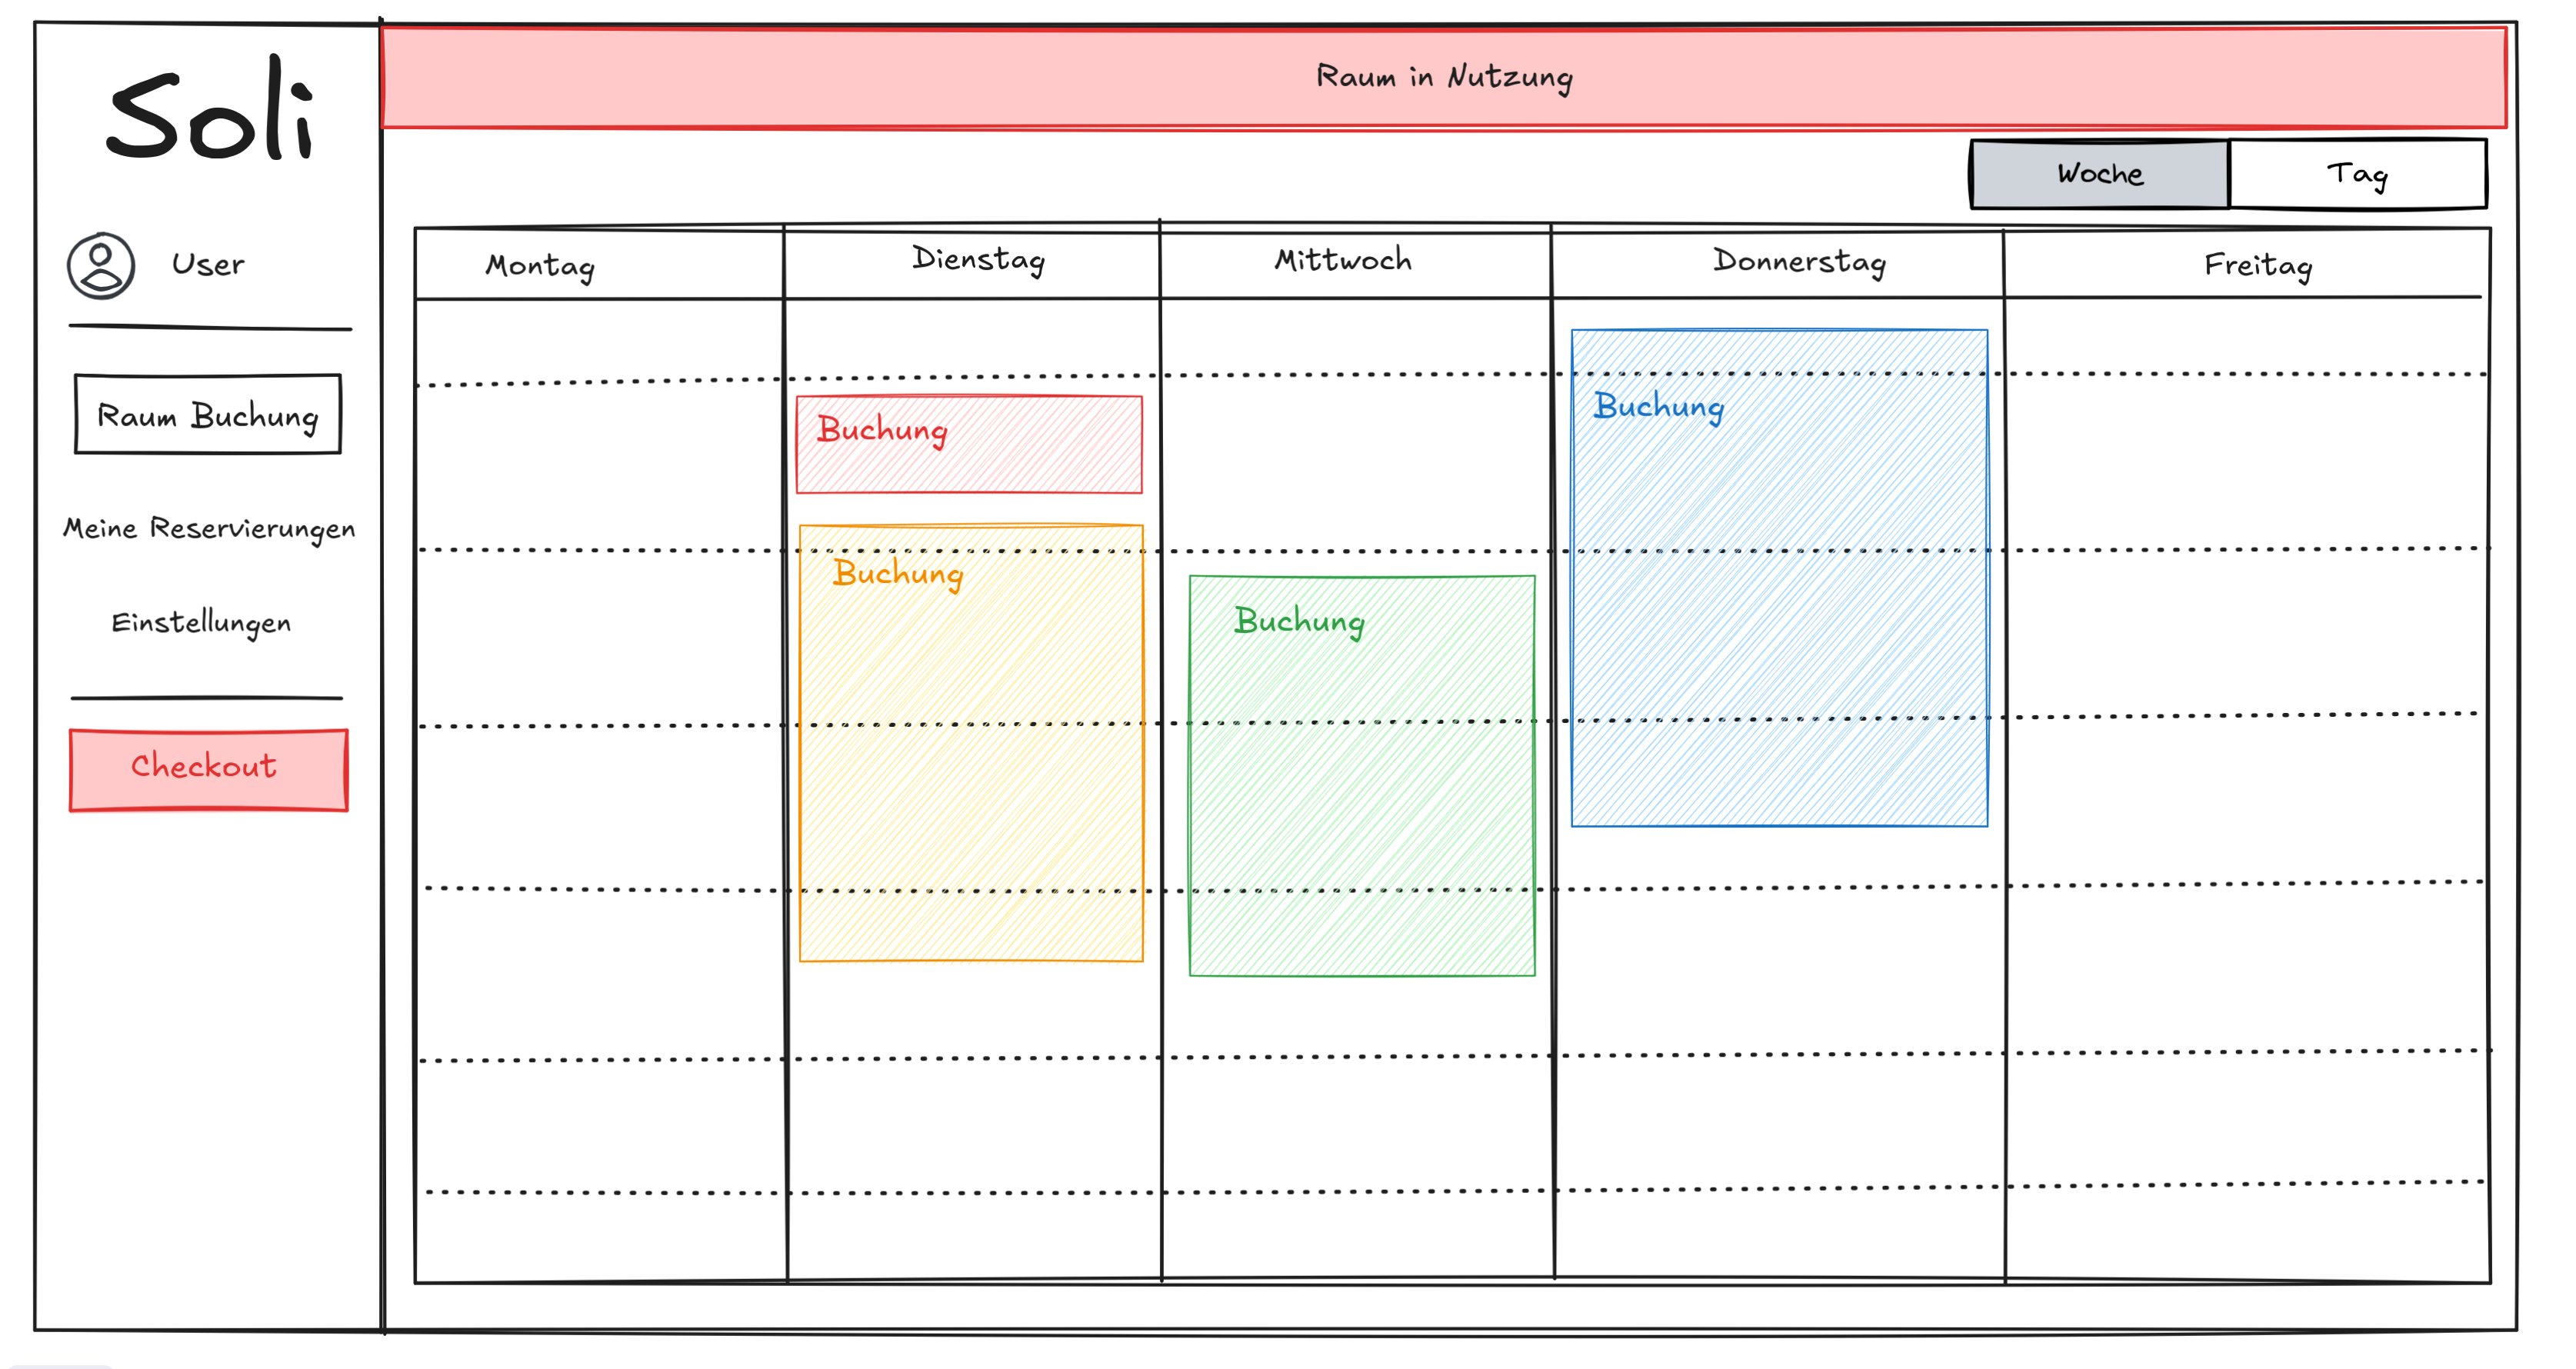
\includegraphics[scale=0.15]{figures/checkout.png}
    \caption{Quick Checkout}
    \label{fig:checkout}
\end{figure}
\pagebreak


\begin{figure}[ht]
    
    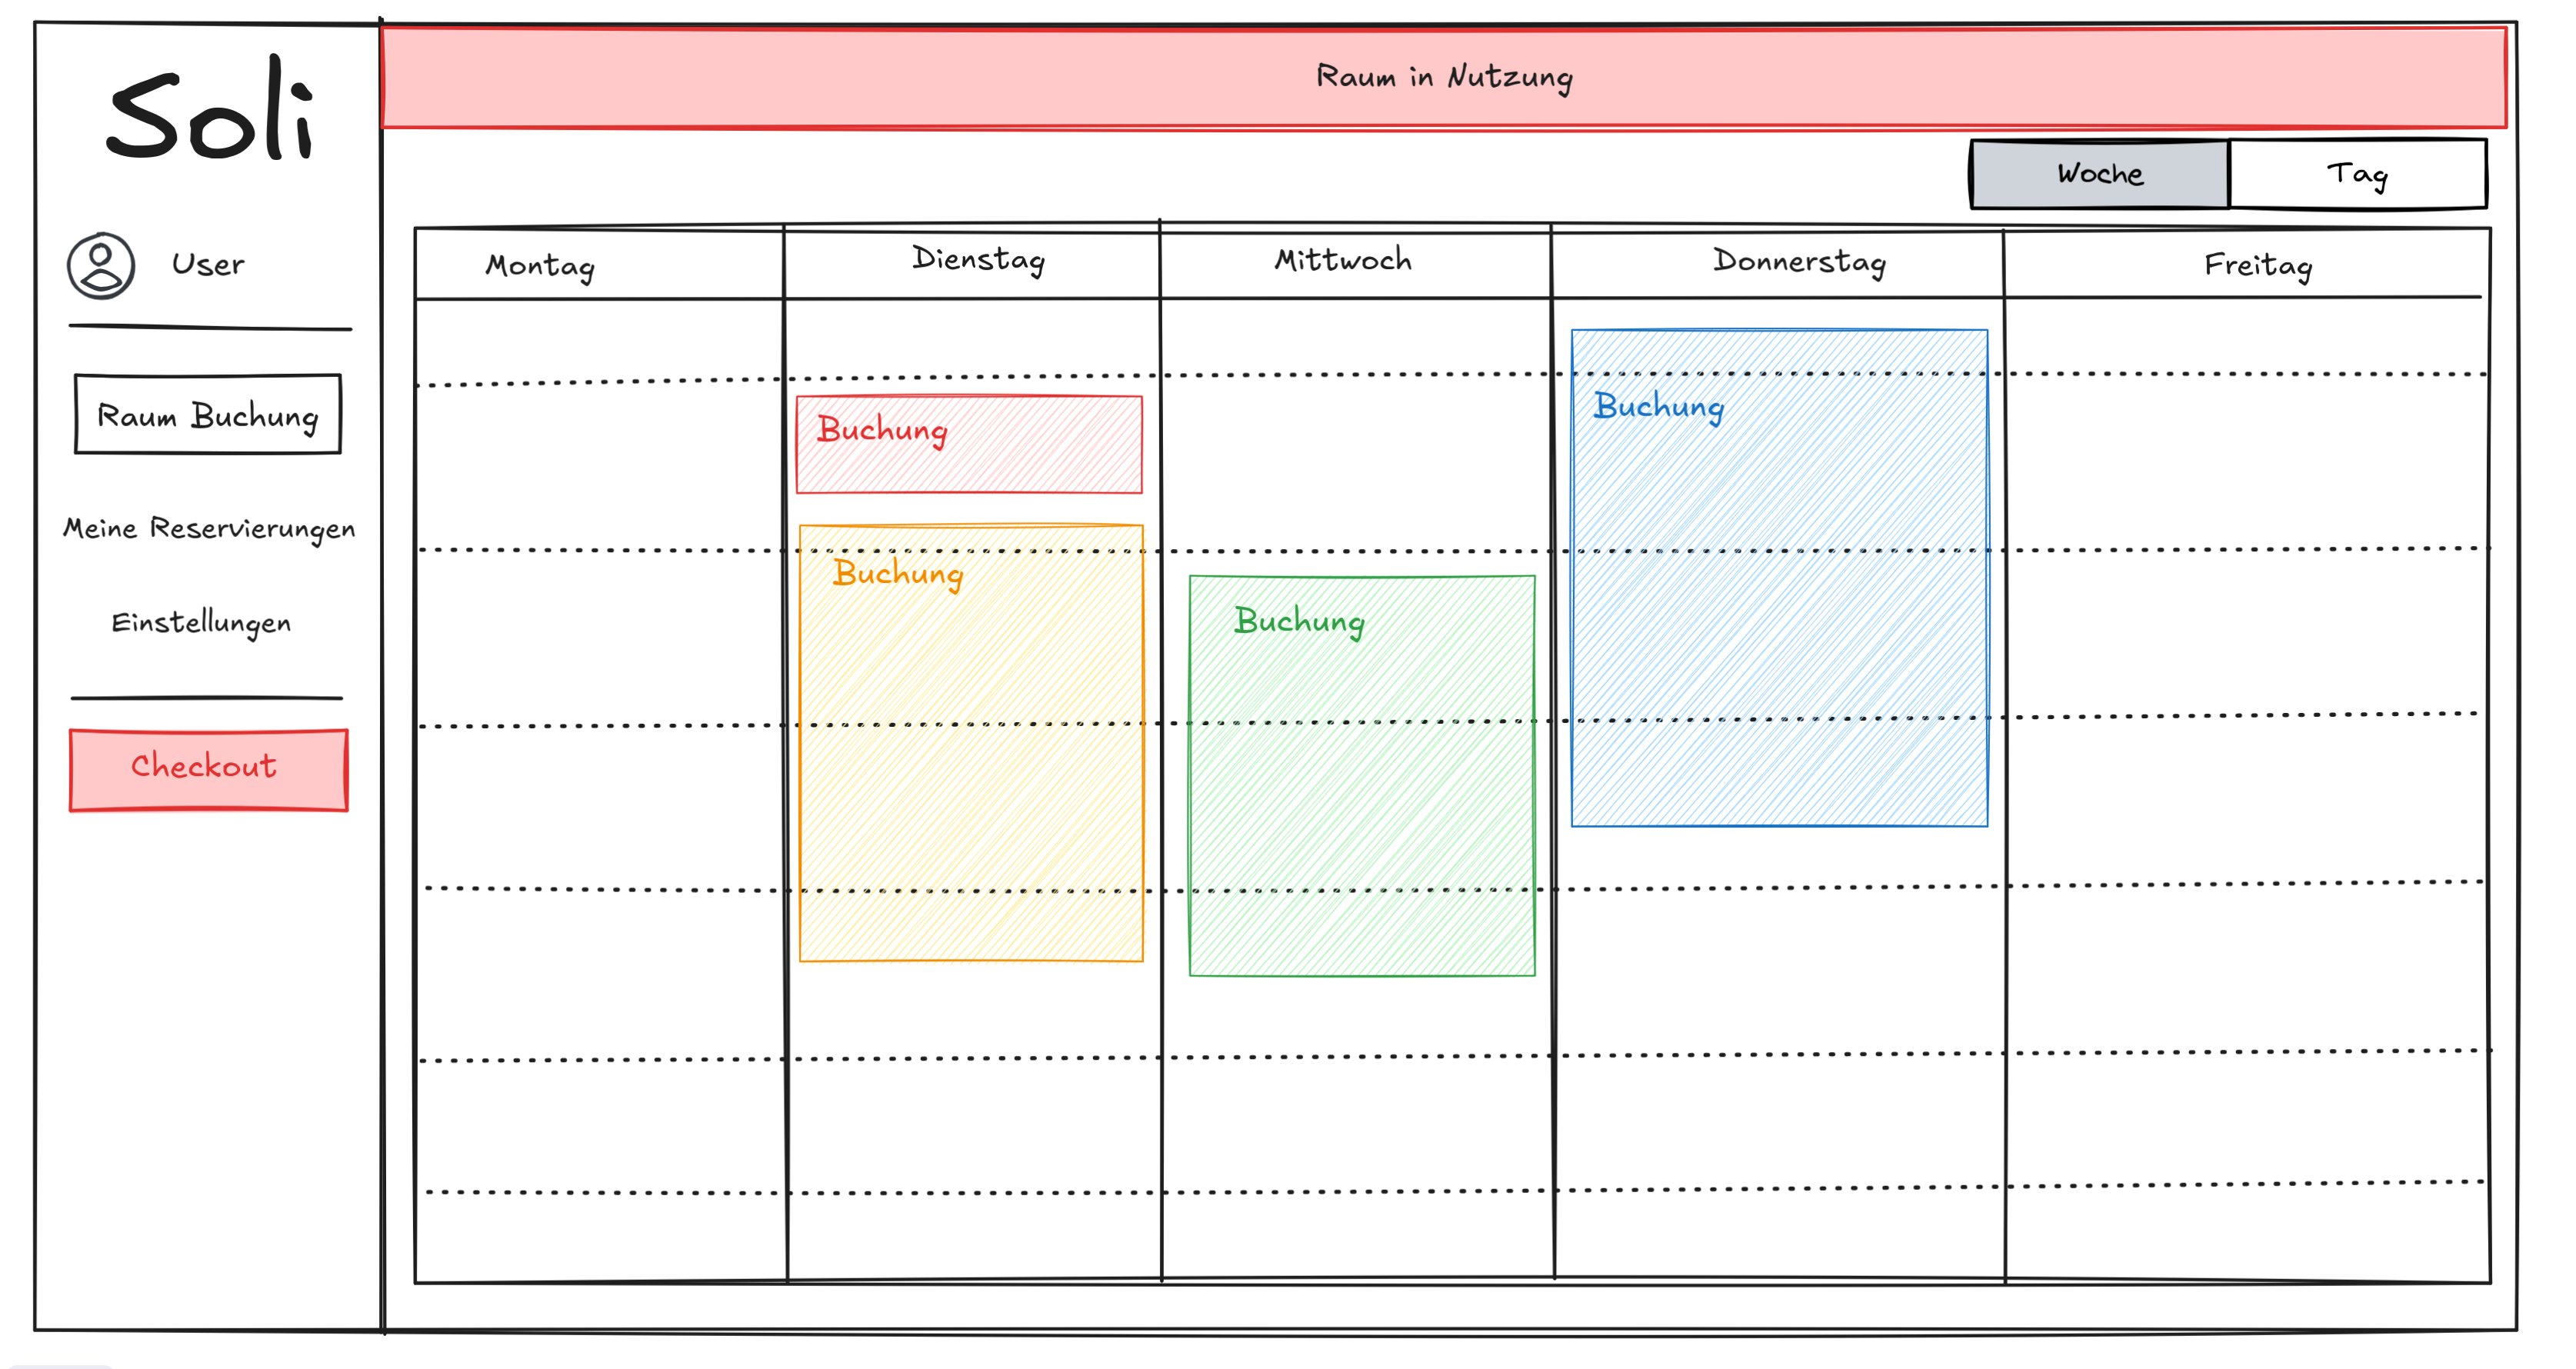
\includegraphics[scale=0.15]{figures/checkout.png}
    \caption{Buchungsverwaltungsansicht}
    \label{fig:fklsj}
\end{figure}
